% Options for packages loaded elsewhere
\PassOptionsToPackage{unicode}{hyperref}
\PassOptionsToPackage{hyphens}{url}
%
\documentclass[
]{article}
\usepackage{lmodern}
\usepackage{amssymb,amsmath}
\usepackage{ifxetex,ifluatex}
\ifnum 0\ifxetex 1\fi\ifluatex 1\fi=0 % if pdftex
  \usepackage[T1]{fontenc}
  \usepackage[utf8]{inputenc}
  \usepackage{textcomp} % provide euro and other symbols
\else % if luatex or xetex
  \usepackage{unicode-math}
  \defaultfontfeatures{Scale=MatchLowercase}
  \defaultfontfeatures[\rmfamily]{Ligatures=TeX,Scale=1}
\fi
% Use upquote if available, for straight quotes in verbatim environments
\IfFileExists{upquote.sty}{\usepackage{upquote}}{}
\IfFileExists{microtype.sty}{% use microtype if available
  \usepackage[]{microtype}
  \UseMicrotypeSet[protrusion]{basicmath} % disable protrusion for tt fonts
}{}
\makeatletter
\@ifundefined{KOMAClassName}{% if non-KOMA class
  \IfFileExists{parskip.sty}{%
    \usepackage{parskip}
  }{% else
    \setlength{\parindent}{0pt}
    \setlength{\parskip}{6pt plus 2pt minus 1pt}}
}{% if KOMA class
  \KOMAoptions{parskip=half}}
\makeatother
\usepackage{xcolor}
\IfFileExists{xurl.sty}{\usepackage{xurl}}{} % add URL line breaks if available
\IfFileExists{bookmark.sty}{\usepackage{bookmark}}{\usepackage{hyperref}}
\hypersetup{
  pdftitle={GVault QDMS Post Go-Live Survey: R Notebook},
  hidelinks,
  pdfcreator={LaTeX via pandoc}}
\urlstyle{same} % disable monospaced font for URLs
\usepackage[margin=1in]{geometry}
\usepackage{color}
\usepackage{fancyvrb}
\newcommand{\VerbBar}{|}
\newcommand{\VERB}{\Verb[commandchars=\\\{\}]}
\DefineVerbatimEnvironment{Highlighting}{Verbatim}{commandchars=\\\{\}}
% Add ',fontsize=\small' for more characters per line
\usepackage{framed}
\definecolor{shadecolor}{RGB}{248,248,248}
\newenvironment{Shaded}{\begin{snugshade}}{\end{snugshade}}
\newcommand{\AlertTok}[1]{\textcolor[rgb]{0.94,0.16,0.16}{#1}}
\newcommand{\AnnotationTok}[1]{\textcolor[rgb]{0.56,0.35,0.01}{\textbf{\textit{#1}}}}
\newcommand{\AttributeTok}[1]{\textcolor[rgb]{0.77,0.63,0.00}{#1}}
\newcommand{\BaseNTok}[1]{\textcolor[rgb]{0.00,0.00,0.81}{#1}}
\newcommand{\BuiltInTok}[1]{#1}
\newcommand{\CharTok}[1]{\textcolor[rgb]{0.31,0.60,0.02}{#1}}
\newcommand{\CommentTok}[1]{\textcolor[rgb]{0.56,0.35,0.01}{\textit{#1}}}
\newcommand{\CommentVarTok}[1]{\textcolor[rgb]{0.56,0.35,0.01}{\textbf{\textit{#1}}}}
\newcommand{\ConstantTok}[1]{\textcolor[rgb]{0.00,0.00,0.00}{#1}}
\newcommand{\ControlFlowTok}[1]{\textcolor[rgb]{0.13,0.29,0.53}{\textbf{#1}}}
\newcommand{\DataTypeTok}[1]{\textcolor[rgb]{0.13,0.29,0.53}{#1}}
\newcommand{\DecValTok}[1]{\textcolor[rgb]{0.00,0.00,0.81}{#1}}
\newcommand{\DocumentationTok}[1]{\textcolor[rgb]{0.56,0.35,0.01}{\textbf{\textit{#1}}}}
\newcommand{\ErrorTok}[1]{\textcolor[rgb]{0.64,0.00,0.00}{\textbf{#1}}}
\newcommand{\ExtensionTok}[1]{#1}
\newcommand{\FloatTok}[1]{\textcolor[rgb]{0.00,0.00,0.81}{#1}}
\newcommand{\FunctionTok}[1]{\textcolor[rgb]{0.00,0.00,0.00}{#1}}
\newcommand{\ImportTok}[1]{#1}
\newcommand{\InformationTok}[1]{\textcolor[rgb]{0.56,0.35,0.01}{\textbf{\textit{#1}}}}
\newcommand{\KeywordTok}[1]{\textcolor[rgb]{0.13,0.29,0.53}{\textbf{#1}}}
\newcommand{\NormalTok}[1]{#1}
\newcommand{\OperatorTok}[1]{\textcolor[rgb]{0.81,0.36,0.00}{\textbf{#1}}}
\newcommand{\OtherTok}[1]{\textcolor[rgb]{0.56,0.35,0.01}{#1}}
\newcommand{\PreprocessorTok}[1]{\textcolor[rgb]{0.56,0.35,0.01}{\textit{#1}}}
\newcommand{\RegionMarkerTok}[1]{#1}
\newcommand{\SpecialCharTok}[1]{\textcolor[rgb]{0.00,0.00,0.00}{#1}}
\newcommand{\SpecialStringTok}[1]{\textcolor[rgb]{0.31,0.60,0.02}{#1}}
\newcommand{\StringTok}[1]{\textcolor[rgb]{0.31,0.60,0.02}{#1}}
\newcommand{\VariableTok}[1]{\textcolor[rgb]{0.00,0.00,0.00}{#1}}
\newcommand{\VerbatimStringTok}[1]{\textcolor[rgb]{0.31,0.60,0.02}{#1}}
\newcommand{\WarningTok}[1]{\textcolor[rgb]{0.56,0.35,0.01}{\textbf{\textit{#1}}}}
\usepackage{graphicx,grffile}
\makeatletter
\def\maxwidth{\ifdim\Gin@nat@width>\linewidth\linewidth\else\Gin@nat@width\fi}
\def\maxheight{\ifdim\Gin@nat@height>\textheight\textheight\else\Gin@nat@height\fi}
\makeatother
% Scale images if necessary, so that they will not overflow the page
% margins by default, and it is still possible to overwrite the defaults
% using explicit options in \includegraphics[width, height, ...]{}
\setkeys{Gin}{width=\maxwidth,height=\maxheight,keepaspectratio}
% Set default figure placement to htbp
\makeatletter
\def\fps@figure{htbp}
\makeatother
\setlength{\emergencystretch}{3em} % prevent overfull lines
\providecommand{\tightlist}{%
  \setlength{\itemsep}{0pt}\setlength{\parskip}{0pt}}
\setcounter{secnumdepth}{-\maxdimen} % remove section numbering

\title{GVault QDMS Post Go-Live Survey: R Notebook}
\author{}
\date{\vspace{-2.5em}}

\begin{document}
\maketitle

\hypertarget{initialize-the-packages}{%
\paragraph{Initialize the packages}\label{initialize-the-packages}}

Remove comments if you haven't installed the packages in R yet.

\begin{Shaded}
\begin{Highlighting}[]
\CommentTok{# install.packages("RcURL")}
\CommentTok{# install.packages("randomForest") }
\CommentTok{# install.packages("e1071")}
\CommentTok{# install.packages("caret")}
\CommentTok{# install.packages("ggplot2")}

\KeywordTok{library}\NormalTok{(RCurl)}
\end{Highlighting}
\end{Shaded}

\begin{verbatim}
## Loading required package: bitops
\end{verbatim}

\begin{Shaded}
\begin{Highlighting}[]
\KeywordTok{library}\NormalTok{(randomForest)  }
\end{Highlighting}
\end{Shaded}

\begin{verbatim}
## randomForest 4.6-14
\end{verbatim}

\begin{verbatim}
## Type rfNews() to see new features/changes/bug fixes.
\end{verbatim}

\begin{Shaded}
\begin{Highlighting}[]
\KeywordTok{library}\NormalTok{(e1071)  }
\KeywordTok{library}\NormalTok{(caret)  }
\end{Highlighting}
\end{Shaded}

\begin{verbatim}
## Loading required package: lattice
\end{verbatim}

\begin{verbatim}
## Loading required package: ggplot2
\end{verbatim}

\begin{verbatim}
## 
## Attaching package: 'ggplot2'
\end{verbatim}

\begin{verbatim}
## The following object is masked from 'package:randomForest':
## 
##     margin
\end{verbatim}

\begin{Shaded}
\begin{Highlighting}[]
\KeywordTok{library}\NormalTok{(ggplot2)  }
\KeywordTok{set.seed}\NormalTok{(}\DecValTok{123}\NormalTok{) }
\end{Highlighting}
\end{Shaded}

Load dataset

\begin{Shaded}
\begin{Highlighting}[]
\NormalTok{df1<-}\KeywordTok{read.csv}\NormalTok{(}\StringTok{"Gvault_survey_raw.csv"}\NormalTok{,}\DataTypeTok{header =}\NormalTok{ T)}
\end{Highlighting}
\end{Shaded}

\hypertarget{data-exploration}{%
\paragraph{Data exploration}\label{data-exploration}}

Drop irrelevant columns

\begin{Shaded}
\begin{Highlighting}[]
\NormalTok{df1 =}\StringTok{ }\KeywordTok{subset}\NormalTok{(df1, }\DataTypeTok{select =} \OperatorTok{-}\KeywordTok{c}\NormalTok{(Respondent.ID,Collector.ID,Start.Date,}
\NormalTok{          End.Date,explain_training_effectiveness,explain_support,}
\NormalTok{          explain_complete_without_help,explain_easy_access_documents,}
\NormalTok{          explain_satisfaction,explain_Gvault_efficiency,explain_Gvault_improved, explain_office_location,explain_job_level) )}
\KeywordTok{head}\NormalTok{(df1)}
\end{Highlighting}
\end{Shaded}

\begin{verbatim}
##                freq_use                 role training_instructor_led
## 1                 Daily       Owner / Author          Instructor Led
## 2  At least once a week             Not Sure                        
## 3                 Daily  Reviewer / Approver          Instructor Led
## 4 At least once a month  Reviewer / Approver          Instructor Led
## 5                 Daily Consumer - Read Only                        
## 6                 Daily  Reviewer / Approver          Instructor Led
##   training_web_based                               training_read no_training
## 1 Web/Computer Based Read & Understood of Procedural Document(s)            
## 2 Web/Computer Based Read & Understood of Procedural Document(s)            
## 3 Web/Computer Based Read & Understood of Procedural Document(s)            
## 4                                                                           
## 5                    Read & Understood of Procedural Document(s)            
## 6 Web/Computer Based Read & Understood of Procedural Document(s)            
##   training_effectiveness support_Gnet   support_inapplication
## 1              Effective                                     
## 2   Not effective enough                                     
## 3              Effective              In-Application (GVault)
## 4              Effective                                     
## 5   Not effective enough                                     
## 6              Effective         GNet                        
##                                                             support_ref_doc
## 1 Reference Document (User Manual, Reference Guide, Training Material, etc)
## 2 Reference Document (User Manual, Reference Guide, Training Material, etc)
## 3 Reference Document (User Manual, Reference Guide, Training Material, etc)
## 4                                                                          
## 5                                                                          
## 6 Reference Document (User Manual, Reference Guide, Training Material, etc)
##                  support_SOP                               support_contacted
## 1 SOPs and Work Instructions Contacted my Document Control or Training Group
## 2                                                                           
## 3                                                                           
## 4 SOPs and Work Instructions                                                
## 5                                                                           
## 6 SOPs and Work Instructions Contacted my Document Control or Training Group
##   support_IT complete_without_help easy_access_documents   satisfaction
## 1                 Most of the time                   Yes      Satisfied
## 2                 Some of the time                   Yes      Satisfied
## 3                 Most of the time                   Yes      Satisfied
## 4                 Most of the time                   Yes Very Satisfied
## 5                     All the time                   Yes Very Satisfied
## 6                 Most of the time                   Yes      Satisfied
##          Gvault_efficiency Gvault_improved
## 1                Increased             Yes
## 2                Increased             Yes
## 3                Increased             Yes
## 4 No noticeable difference             Yes
## 5 No noticeable difference                
## 6                Increased             Yes
##                                      functional_area explain_functional_area
## 1 Pharmaceutical Development and Manufacturing (PDM)                        
## 2                     Research and Development (R&D)                        
## 3 Pharmaceutical Development and Manufacturing (PDM)                        
## 4                          Facilities and Operations                        
## 5                     Research and Development (R&D)                        
## 6 Pharmaceutical Development and Manufacturing (PDM)                        
##   office_location              job_level time_worked_Glead
## 1     Foster City Manager / Group Leader          >7 Years
## 2       Cambridge               Director          >7 Years
## 3     Foster City Individual Contributor  Less than a year
## 4     Foster City Individual Contributor      1 to 2 years
## 5     Foster City Individual Contributor  Less than a year
## 6         Alberta Manager / Group Leader          >7 Years
\end{verbatim}

Explore the data before fitting a model to get an idea of what to
expect. I am plotting a variable on two axes and using colors to see the
relationship among the levels of satisfaction. Lets explore the
relationship between satisfaction and frequency of use

\begin{Shaded}
\begin{Highlighting}[]
\NormalTok{p=}\KeywordTok{ggplot}\NormalTok{(df1,}\KeywordTok{aes}\NormalTok{(}\DataTypeTok{x=}\NormalTok{df1}\OperatorTok{$}\NormalTok{freq_use,}\DataTypeTok{y=}\NormalTok{df1}\OperatorTok{$}\NormalTok{satisfaction,}
                 \DataTypeTok{color=}\NormalTok{df1}\OperatorTok{$}\NormalTok{satisfaction),}\DataTypeTok{width=}\DecValTok{80}\NormalTok{,}\DataTypeTok{height=}\DecValTok{60}\NormalTok{)}\OperatorTok{+}
\StringTok{  }\KeywordTok{theme}\NormalTok{(}\DataTypeTok{axis.text.x =} \KeywordTok{element_text}\NormalTok{(}\DataTypeTok{angle =} \DecValTok{90}\NormalTok{))}

\NormalTok{p }\OperatorTok{+}\StringTok{ }\KeywordTok{geom_jitter}\NormalTok{(}\DataTypeTok{alpha=}\FloatTok{0.3}\NormalTok{) }\OperatorTok{+}\StringTok{  }
\StringTok{  }\KeywordTok{scale_color_manual}\NormalTok{(}\DataTypeTok{breaks =} \KeywordTok{c}\NormalTok{(}\StringTok{'Satisfied'}\NormalTok{,}\StringTok{'Very Unsatisfied'}\NormalTok{,}\StringTok{'Very Satisfied'}\NormalTok{,}\StringTok{'Slightly Unsatisfied'}\NormalTok{),}
                     \DataTypeTok{values=}\KeywordTok{c}\NormalTok{(}\StringTok{'darkgreen'}\NormalTok{,}\StringTok{'red'}\NormalTok{,}\StringTok{'blue'}\NormalTok{,}\StringTok{'yellow'}\NormalTok{))}
\end{Highlighting}
\end{Shaded}

\includegraphics{my-first-notebook_files/figure-latex/unnamed-chunk-4-1.pdf}

A comparison of Frequency of use (freq\_use) \& effectiveness of
training to satisfaction shows us: Users who used Gvault daily were more
likely to be satisfied or very satisfied. I'm looking for spots where
there exists an overwhelming majority of one color.

\begin{Shaded}
\begin{Highlighting}[]
\NormalTok{p1=}\KeywordTok{ggplot}\NormalTok{(df1,}\KeywordTok{aes}\NormalTok{(}\DataTypeTok{x=}\NormalTok{df1}\OperatorTok{$}\NormalTok{freq_use,}\DataTypeTok{y=}\NormalTok{df1}\OperatorTok{$}\NormalTok{training_effectiveness,}\DataTypeTok{color=}\NormalTok{df1}\OperatorTok{$}\NormalTok{satisfaction),}\DataTypeTok{width=}\DecValTok{80}\NormalTok{,}\DataTypeTok{height=}\DecValTok{60}\NormalTok{)}\OperatorTok{+}\KeywordTok{theme}\NormalTok{(}\DataTypeTok{axis.text.x =} \KeywordTok{element_text}\NormalTok{(}\DataTypeTok{angle =} \DecValTok{90}\NormalTok{))}
\NormalTok{p1 }\OperatorTok{+}\StringTok{ }\KeywordTok{geom_jitter}\NormalTok{(}\DataTypeTok{alpha=}\FloatTok{0.3}\NormalTok{) }\OperatorTok{+}\StringTok{  }
\StringTok{  }\KeywordTok{scale_color_manual}\NormalTok{(}\DataTypeTok{breaks =} \KeywordTok{c}\NormalTok{(}\StringTok{'Satisfied'}\NormalTok{,}\StringTok{'Very Unsatisfied'}\NormalTok{,}\StringTok{'Very Satisfied'}\NormalTok{,}\StringTok{'Slightly Unsatisfied'}\NormalTok{),}
                     \DataTypeTok{values=}\KeywordTok{c}\NormalTok{(}\StringTok{'darkgreen'}\NormalTok{,}\StringTok{'red'}\NormalTok{,}\StringTok{'blue'}\NormalTok{,}\StringTok{'yellow'}\NormalTok{))}
\end{Highlighting}
\end{Shaded}

\includegraphics{my-first-notebook_files/figure-latex/unnamed-chunk-5-1.pdf}

A comparison of role and the rate of completing work without help in
terms likelihood of satisfaction show that: Reveiwer/Approver role users
completed work in Gvault without help all the time and were more likely
to be satisfied

\begin{Shaded}
\begin{Highlighting}[]
\NormalTok{p1=}\KeywordTok{ggplot}\NormalTok{(df1,}\KeywordTok{aes}\NormalTok{(}\DataTypeTok{y=}\NormalTok{df1}\OperatorTok{$}\NormalTok{role,}\DataTypeTok{x=}\NormalTok{df1}\OperatorTok{$}\NormalTok{complete_without_help,}
\DataTypeTok{color=}\NormalTok{df1}\OperatorTok{$}\NormalTok{satisfaction),}\DataTypeTok{width=}\DecValTok{80}\NormalTok{,}\DataTypeTok{height=}\DecValTok{60}\NormalTok{)}\OperatorTok{+}\KeywordTok{theme}\NormalTok{(}\DataTypeTok{axis.text.x =} \KeywordTok{element_text}\NormalTok{(}\DataTypeTok{angle =} \DecValTok{90}\NormalTok{))}
\NormalTok{p1 }\OperatorTok{+}\StringTok{ }\KeywordTok{geom_jitter}\NormalTok{(}\DataTypeTok{alpha=}\FloatTok{0.3}\NormalTok{) }\OperatorTok{+}\StringTok{  }
\StringTok{  }\KeywordTok{scale_color_manual}\NormalTok{(}\DataTypeTok{breaks =} \KeywordTok{c}\NormalTok{(}\StringTok{'Satisfied'}\NormalTok{,}\StringTok{'Very Unsatisfied'}\NormalTok{,}\StringTok{'Very Satisfied'}\NormalTok{,}\StringTok{'Slightly Unsatisfied'}\NormalTok{),}
                 \DataTypeTok{values=}\KeywordTok{c}\NormalTok{(}\StringTok{'darkgreen'}\NormalTok{,}\StringTok{'red'}\NormalTok{,}\StringTok{'blue'}\NormalTok{,}\StringTok{'yellow'}\NormalTok{))}
\end{Highlighting}
\end{Shaded}

\includegraphics{my-first-notebook_files/figure-latex/unnamed-chunk-6-1.pdf}

\hypertarget{train-test-split}{%
\paragraph{Train test split}\label{train-test-split}}

Create data for training

\begin{Shaded}
\begin{Highlighting}[]
\NormalTok{sample.ind =}\StringTok{ }\KeywordTok{sample}\NormalTok{(}\DecValTok{2}\NormalTok{,}\KeywordTok{nrow}\NormalTok{(df1),}\DataTypeTok{replace =}\NormalTok{ T,}\DataTypeTok{prob =} \KeywordTok{c}\NormalTok{(}\FloatTok{0.9}\NormalTok{,}\FloatTok{0.1}\NormalTok{))}
\NormalTok{data.dev =}\StringTok{ }\NormalTok{df1[sample.ind}\OperatorTok{==}\DecValTok{1}\NormalTok{,]  }
\NormalTok{data.val =}\StringTok{ }\NormalTok{df1[sample.ind}\OperatorTok{==}\DecValTok{2}\NormalTok{,]}
\end{Highlighting}
\end{Shaded}

I wanted to know the split of satisfaction levels in the data set and
compare it between the training and test data.

\begin{Shaded}
\begin{Highlighting}[]
\CommentTok{# Original Data}
\KeywordTok{table}\NormalTok{(df1}\OperatorTok{$}\NormalTok{satisfaction)}\OperatorTok{/}\KeywordTok{nrow}\NormalTok{(df1)}
\end{Highlighting}
\end{Shaded}

\begin{verbatim}
## 
##            Satisfied Slightly Unsatisfied       Very Satisfied 
##           0.56842105           0.14947368           0.23157895 
##     Very Unsatisfied 
##           0.05052632
\end{verbatim}

\begin{Shaded}
\begin{Highlighting}[]
\CommentTok{# Training Data}
\KeywordTok{table}\NormalTok{(data.dev}\OperatorTok{$}\NormalTok{satisfaction)}\OperatorTok{/}\KeywordTok{nrow}\NormalTok{(data.dev)}
\end{Highlighting}
\end{Shaded}

\begin{verbatim}
## 
##            Satisfied Slightly Unsatisfied       Very Satisfied 
##           0.56206089           0.16159251           0.22716628 
##     Very Unsatisfied 
##           0.04918033
\end{verbatim}

\begin{Shaded}
\begin{Highlighting}[]
\CommentTok{# Testing Data}
\KeywordTok{table}\NormalTok{(data.val}\OperatorTok{$}\NormalTok{satisfaction)}\OperatorTok{/}\KeywordTok{nrow}\NormalTok{(data.val) }
\end{Highlighting}
\end{Shaded}

\begin{verbatim}
## 
##            Satisfied Slightly Unsatisfied       Very Satisfied 
##           0.62500000           0.04166667           0.27083333 
##     Very Unsatisfied 
##           0.06250000
\end{verbatim}

\hypertarget{model-training-fit-random-forest-model}{%
\paragraph{Model Training: Fit Random Forest
Model}\label{model-training-fit-random-forest-model}}

I finally fit the random forest model to the training data. Plotting the
model shows us that after about 20 trees, not much changes in terms of
error. It fluctuates a bit but not to a large degree.

\begin{Shaded}
\begin{Highlighting}[]
\NormalTok{rf =}\StringTok{ }\KeywordTok{randomForest}\NormalTok{(satisfaction }\OperatorTok{~}\StringTok{ }\NormalTok{.,}\DataTypeTok{ntree =} \DecValTok{100}\NormalTok{,}\DataTypeTok{data =}\NormalTok{ data.dev)}
\KeywordTok{plot}\NormalTok{(rf)}
\end{Highlighting}
\end{Shaded}

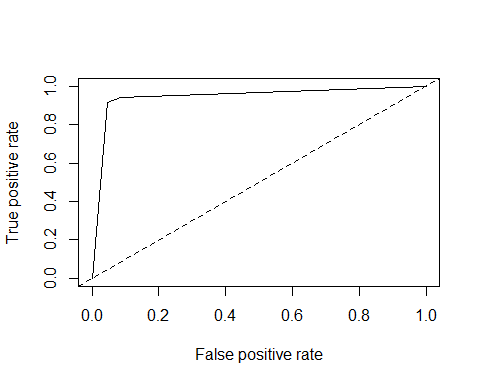
\includegraphics{my-first-notebook_files/figure-latex/unnamed-chunk-11-1.pdf}

\hypertarget{feature-selection-variable-importance}{%
\paragraph{Feature selection: Variable
Importance}\label{feature-selection-variable-importance}}

Training effectiveness is the most important variable in terms of ``Mean
Decreasing Gini'' -- a similar term for information gain.

\begin{Shaded}
\begin{Highlighting}[]
\KeywordTok{varImpPlot}\NormalTok{(rf, }\DataTypeTok{sort =}\NormalTok{ T, }\DataTypeTok{n.var=}\DecValTok{10}\NormalTok{,}\DataTypeTok{main=}\StringTok{"Top 10 - Variable Importance"}\NormalTok{)}
\end{Highlighting}
\end{Shaded}

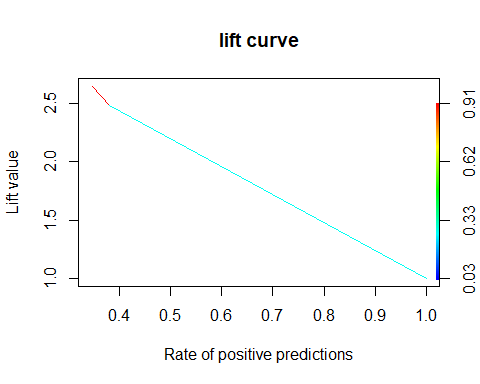
\includegraphics{my-first-notebook_files/figure-latex/unnamed-chunk-12-1.pdf}

\begin{Shaded}
\begin{Highlighting}[]
\NormalTok{var.imp =}\StringTok{ }\KeywordTok{data.frame}\NormalTok{(}\KeywordTok{importance}\NormalTok{(rf, }\DataTypeTok{type=}\DecValTok{2}\NormalTok{))}
\CommentTok{# make row names as columns}
\NormalTok{var.imp}\OperatorTok{$}\NormalTok{Variables =}\StringTok{ }\KeywordTok{row.names}\NormalTok{(var.imp)  }
\KeywordTok{print}\NormalTok{(var.imp[}\KeywordTok{order}\NormalTok{(var.imp}\OperatorTok{$}\NormalTok{MeanDecreaseGini,}\DataTypeTok{decreasing =}\NormalTok{ T),])}
\end{Highlighting}
\end{Shaded}

\begin{verbatim}
##                         MeanDecreaseGini               Variables
## training_effectiveness         21.285491  training_effectiveness
## office_location                20.574519         office_location
## time_worked_Glead              19.654643       time_worked_Glead
## Gvault_improved                19.349842         Gvault_improved
## Gvault_efficiency              18.195220       Gvault_efficiency
## complete_without_help          16.239664   complete_without_help
## job_level                      16.090225               job_level
## role                           15.298479                    role
## easy_access_documents          14.628286   easy_access_documents
## functional_area                14.518986         functional_area
## freq_use                       12.622863                freq_use
## support_ref_doc                 6.735509         support_ref_doc
## support_inapplication           6.655658   support_inapplication
## support_Gnet                    6.396340            support_Gnet
## support_SOP                     6.385338             support_SOP
## support_contacted               6.127248       support_contacted
## training_instructor_led         5.917755 training_instructor_led
## training_read                   5.645961           training_read
## training_web_based              5.619668      training_web_based
## explain_functional_area         3.812994 explain_functional_area
## support_IT                      3.025611              support_IT
## no_training                     1.363020             no_training
\end{verbatim}

\hypertarget{prediction-and-model-evaluation}{%
\paragraph{Prediction and Model
Evaluation}\label{prediction-and-model-evaluation}}

I decided to use the model to attempt to predict the satisfaction level
based off of the training data set. It predicted the response variable
perfectly -- having zero false positives or false negatives.

\begin{Shaded}
\begin{Highlighting}[]
\CommentTok{# Predicting response variable}
\NormalTok{data.dev}\OperatorTok{$}\NormalTok{predicted.response =}\StringTok{ }\KeywordTok{predict}\NormalTok{(rf , data.dev)}

\CommentTok{# Create Confusion Matrix}
\KeywordTok{print}\NormalTok{(}\KeywordTok{confusionMatrix}\NormalTok{(}\DataTypeTok{data =}\NormalTok{ data.dev}\OperatorTok{$}\NormalTok{predicted.response,  }
                  \DataTypeTok{reference =}\NormalTok{ data.dev}\OperatorTok{$}\NormalTok{satisfaction,}
                  \DataTypeTok{positive =}\StringTok{'Very Satisfied'}\NormalTok{))}
\end{Highlighting}
\end{Shaded}

\begin{verbatim}
## Confusion Matrix and Statistics
## 
##                       Reference
## Prediction             Satisfied Slightly Unsatisfied Very Satisfied
##   Satisfied                  240                    0              2
##   Slightly Unsatisfied         0                   69              0
##   Very Satisfied               0                    0             95
##   Very Unsatisfied             0                    0              0
##                       Reference
## Prediction             Very Unsatisfied
##   Satisfied                           0
##   Slightly Unsatisfied                0
##   Very Satisfied                      0
##   Very Unsatisfied                   21
## 
## Overall Statistics
##                                           
##                Accuracy : 0.9953          
##                  95% CI : (0.9832, 0.9994)
##     No Information Rate : 0.5621          
##     P-Value [Acc > NIR] : < 2.2e-16       
##                                           
##                   Kappa : 0.9922          
##                                           
##  Mcnemar's Test P-Value : NA              
## 
## Statistics by Class:
## 
##                      Class: Satisfied Class: Slightly Unsatisfied
## Sensitivity                    1.0000                      1.0000
## Specificity                    0.9893                      1.0000
## Pos Pred Value                 0.9917                      1.0000
## Neg Pred Value                 1.0000                      1.0000
## Prevalence                     0.5621                      0.1616
## Detection Rate                 0.5621                      0.1616
## Detection Prevalence           0.5667                      0.1616
## Balanced Accuracy              0.9947                      1.0000
##                      Class: Very Satisfied Class: Very Unsatisfied
## Sensitivity                         0.9794                 1.00000
## Specificity                         1.0000                 1.00000
## Pos Pred Value                      1.0000                 1.00000
## Neg Pred Value                      0.9940                 1.00000
## Prevalence                          0.2272                 0.04918
## Detection Rate                      0.2225                 0.04918
## Detection Prevalence                0.2225                 0.04918
## Balanced Accuracy                   0.9897                 1.00000
\end{verbatim}

\hypertarget{model-testing}{%
\paragraph{Model Testing}\label{model-testing}}

Now it was time to see how the model did with data it had not seen
before-- making predictions on the test data. It did a decent job. It
had a 71\% accuracy with a very narrow confidence interval. It did have
3 false negatives:6.6\% and 6 false positives:13.3\% (which could be
slightly missleading \# if you were actually predicting satisfaction
based on this model).

\begin{Shaded}
\begin{Highlighting}[]
\CommentTok{# Predicting response variable}
\NormalTok{data.val}\OperatorTok{$}\NormalTok{predicted.response <-}\StringTok{ }\KeywordTok{predict}\NormalTok{(rf ,data.val)}

\CommentTok{# Create Confusion Matrix}
\KeywordTok{print}\NormalTok{(}\KeywordTok{confusionMatrix}\NormalTok{(}\DataTypeTok{data=}\NormalTok{data.val}\OperatorTok{$}\NormalTok{predicted.response,  }
                  \DataTypeTok{reference=}\NormalTok{data.val}\OperatorTok{$}\NormalTok{satisfaction,}
                  \DataTypeTok{positive=}\StringTok{'Very Satisfied'}\NormalTok{))}
\end{Highlighting}
\end{Shaded}

\begin{verbatim}
## Confusion Matrix and Statistics
## 
##                       Reference
## Prediction             Satisfied Slightly Unsatisfied Very Satisfied
##   Satisfied                   26                    1              8
##   Slightly Unsatisfied         3                    1              0
##   Very Satisfied               1                    0              5
##   Very Unsatisfied             0                    0              0
##                       Reference
## Prediction             Very Unsatisfied
##   Satisfied                           0
##   Slightly Unsatisfied                3
##   Very Satisfied                      0
##   Very Unsatisfied                    0
## 
## Overall Statistics
##                                          
##                Accuracy : 0.6667         
##                  95% CI : (0.5159, 0.796)
##     No Information Rate : 0.625          
##     P-Value [Acc > NIR] : 0.3313         
##                                          
##                   Kappa : 0.3391         
##                                          
##  Mcnemar's Test P-Value : NA             
## 
## Statistics by Class:
## 
##                      Class: Satisfied Class: Slightly Unsatisfied
## Sensitivity                    0.8667                     0.50000
## Specificity                    0.5000                     0.86957
## Pos Pred Value                 0.7429                     0.14286
## Neg Pred Value                 0.6923                     0.97561
## Prevalence                     0.6250                     0.04167
## Detection Rate                 0.5417                     0.02083
## Detection Prevalence           0.7292                     0.14583
## Balanced Accuracy              0.6833                     0.68478
##                      Class: Very Satisfied Class: Very Unsatisfied
## Sensitivity                         0.3846                  0.0000
## Specificity                         0.9714                  1.0000
## Pos Pred Value                      0.8333                     NaN
## Neg Pred Value                      0.8095                  0.9375
## Prevalence                          0.2708                  0.0625
## Detection Rate                      0.1042                  0.0000
## Detection Prevalence                0.1250                  0.0000
## Balanced Accuracy                   0.6780                  0.5000
\end{verbatim}

\end{document}
